\section{Introduction}
%rewrite intro
Climate change mitigation goals require profound changes in socioeconomic production systems. This is especially true for the energy system (electricity and heat generation), which is responsible for 15.5 Gt CO2 emissions in 2021, or 43\% of energy-related CO2 emissions (\cite{IEA2021}). Emissions from the power generation sector come from the combustion of fossil resources, namely coal, oil, and gas, in existing power plants. It is now widely recognized that achieving ambitious decarbonization targets requires a rapid phase-out of fossil fuel combustion. However, given the inertia of capital in this sector (power plants are expected to operate for decades), today's option for power generation is determined by the capacity built in the past. Therefore, an accurate representation of power generation capacity expansion decisions is key to capturing current and future power system developments needed to address climate change.



The presentation of the main characteristics of electricity systems ultimately requires consideration of two types of decisions made under techno-economic constraints:
\begin{enumerate}
    \item the long-term choice of optimal capacity to match future electricity demand (invetment)
    \item the short-term choice of capacity utilization to supply current load (dispatch)
\end{enumerate}
The investment and dispatch decisions are addressed in separate sub-modules of the electricity module (or electricity nexus) of IMACLIM-R. Note that in our framework, the electricity sector refers to the sector in the macroeconomic core of IMACLIM-R, while the electricity module or nexus refers to its dynamic, bottom-up counterpart.

Below, one will learn more about the modeling framework for investment and dispatch decisions. We begin with a characterization of the technical and economic conditions of electricity generation: \textbf{section 2} describes the technical and cost assumptions underlying the choice of electricity generation capacity, while \textbf{section 3} presents the inclusion of demand-side and renewable energy generation constraints. The next sections detail the investment (\textbf{section 4}) and dispatch (\textbf{section 5}) decision frameworks. \textbf{Section 6} details the link between the electricity nexus and the rest of the economy, while \textbf{section 7} presents the main results of the nexus.

\part*{A bottom-up description of electricity generation conditions}

\section{Explicit electricity generation technologies described in terms of capital generation}

\paragraph {Cost assumptions and technical change in the electricity sector.} In the current version of IMACLIM-R, 20 technologies are available for investment in electricity generation. Each of the 20 technologies is characterized by a set of techno-economic parameters that can be used to calculate the levelized cost of electricity (LCOE). These parameters include: Investment costs, energy efficiency, fixed and variable operation and maintenance costs, an availability factor for dispatchable technologies (in \% of full load hours), a capacity factor for non-dispatchable technologies (in \% of full load hours), lifetimes, and a discount rate that includes both the opportunity cost of capital and a unique risk factor for each technology (Briera and Lefèvre, in prep.).

The techno-economic parameters for each technology are calibrated using sectoral technology models or information from the literature (\cite{IEA2020}, \cite{IRENA2020})
For immature technologies, costs decrease over time through a global learning process modeled by learning curves (\cite{Neij2008}). Learning curves link production costs to cumulative production through a learning coefficient. In the case of the electricity sector, the cost of electricity production is expected to decrease with cumulative installed capacity for a given technology. In the base year of the model (2014), all regions in the IMACLIM-R model start with different cost assumptions. In addition, minimum costs are defined in each region: these are the lowest costs that can be achieved through a learning process. As a result, the learning process is global (each region benefits from the capacity additions of the others), but the initial and asymptotic costs remain differentiated. This decision is justified by two findings: 1) wind turbines and PV modules are traded as commodities. 2) capital costs varies by location due to national or regional circumstances, such as labor costs. With $CINV_{k,j}(t)$ the current investment cost for technology $j$ in region $k$ at time $t$, $CINV$\textunderscore $ref_{k,j}$, the reference investment cost (at calibration year), $A$\textunderscore$CINV$\textunderscore$ref_{k,j}$ the floor cost, $LR_{j}$ the learning rate, $Cum$\textunderscore$Inv$\textunderscore$ref_{k,j}$ the cumulative investment of technology $j$ in region $k$ in the calibration year, $Cum$\textunderscore $Inv_{k,j}(t)$ the cumulative investment at time $t$:

\begin{dmath}
    CINV_{k,j}(t) = max(A\_CINV \_ ref_{k,j}, CINV\_ref_{k,j}*(1-LR_{j})^{log(\frac{Cum\_Inv_{k,j}(t)}{Cum\_Inv\_ ref_{k,j}})})
    \label{eqn:LR}
\end{dmath}

As the cost of renewable energy has declined recently, the CAPEX and OPEX curves for wind and solar (including CSP) are driven to adjust to recently observed levels in the region. This means that the decline in renewable energy costs between 2014 and 2019 is monitored and not driven by the learning curve.

\paragraph{Carbon Capture and Storage.}
The electricity nexus of IMACLIM-R includes both fossil fuel carbon capture and storage (CCS) and bioenergy with CCS (BECCS) technologies. In the current version of the model, CCS for power generation technologies does not enter the R\&D phase until a threshold for the current regional carbon price is reached to prevent early CCS deployment despite low or negative profitability. The market share of each CCS technology is limited by an S-shaped technology development function. In the case of BECCS, an additional biomass supply curve limits the deployment of this technology (\cite{Hoogwijk2009}). In the current structure of IMACLIM-R, BECCS are the only source of negative emissions. Therefore, the pace of BECCS deployment is critical in very low-carbon/net-zero mitigation pathways. Fossil fuel technologies cannot be retrofitted with CCS, so new power plants must be built to capture and store carbon. Retrofits and early decomissionning will be added in future versions of the model.


\paragraph{Capital inertia.}
In the electricity sector, the capital stock is path-dependent, as each investment at time t adds to the capacity built in previous periods. The variable $Cap$ \textunderscore $vintage_{k,j}(t)$ tracks annual capacity additions for technology $j$ in region $k$. Thus, the depreciated capital at time $t$ is the sum of the generations of capital that reach the end of their lives from time $t - lifetime$ to $t - 1$ $(Cap$\textunderscore$dep_{k,j}(t)$ in Equation \ref{eqn:Cap_elec_dep}). Adding the new investments to the depreciated capital stock at time t gives the functioning capital at time t before the new capacity addition from the investments.
\begin{dmath}
    Cap\_vintage_{k,j}(t) = Inv_{k,j}(t)
    \label{eqn:Cap_elec_vintage}
\end{dmath}

\begin{dmath}
    Cap \_ dep_{k,j}(t) = \sum_{i = t - lifetime_{k}}^{t-1}Cap\_vintage_{k,j}(i)
    \label{eqn:Cap_elec_dep}
\end{dmath}

\begin{dmath}
    Cap_{k,j}(t) = Cap\_dep_{k,j}(t) + Inv_{k,j}(t)
    \label{eqn:Cap_elec}
\end{dmath}




At each time step of the model, the average characteristics of installed production capacity are the weighted average of the technical characteristics of the different generations of power plants still in operation.
The inertia of power plant capacity is represented by the tracking of capital across generations along with their technical characteristics.

Each year, the production units that reach the end of their life are decommissioned.
If we add the annual capacity additions $i.e.$ investments, we get a net installed capacity.

The new generation of capital capacity and its technical characteristics are determined by the investment decisions described in the following sections.
\section{A challenge to incorporate demand-side and renewable energy supply constraints in a compact electricity module}

\paragraph{Final energy demand in IMACLIM-R.}

In IMACLIM-R, final energy demand results from three (meta) sectors: productive sectors, transport sectors, and the residential sector. For the transport and the residential sectors, which benefit from detailed bottom-up representations, the use of electricity depends on explicit technology choices, $e.g.$ the purchase of electric cars instead of internal combustion engine cars. In the case of productive sectors (agriculture, industry, construction, composite goods), electricity demand is determined by input-output coefficients.

\paragraph{The load duration curve.}


It is common to combine the daily load curves over the 365 days of the year into a single curve, the load duration curve. It summarizes information about the size and degree of utilization of the capacity needed to meet demand throughout the year.
The load duration curve is obtained by plotting hourly load values over the year against the duration for which that load was requested. The highest recorded load over the 8760 hours of the year is called the peak load. The minimum power supplied over the year is the base load. Thus, the balance between electricity demand and supply can be resolved annually using the load duration curve. It allows not relying on an external high-resolution energy model, but it also has its pitfalls, especially in terms of information losses in intraday processes such as short-term storage. These limitations are overcome by integrating additional bottom-up data into the nexus (see subsection "The Residual Load Duration Curve and the challenges to VRE integration").

The shape of the load duration curve is specific to each region, as it is directly related to the temporal variability of electricity demand. This variability depends in particular on the seasonal climate variations in the region
For numerical simplicity, the regional load duration curves were approximated by segmented linear functions:
\begin{itemize}
    \item the possible annual loads (measured in hours) are divided into seven intervals with the following boundaries: [0, 730, 2190, 3650, 5110, 6570, 8030, 8760];
    \item the maximum load lasts 730 hours (peak load);
    \item the minimum load lasts 8760 hours (base load);
    \item the load level for the other periods of time is calculated by dividing the interval between baseload and peak load into six equal segments $i.e.$ 760 hours of baseload, 760 hours of peak load, and five segments in between of 1460 hours each.
\end{itemize}

This results in the shape of the load duration curve in Figure \ref{fig:LDC}: a peak load band, 5 inner load bands, and a base load band.
With this simplified scheme, the load duration curve of each region can be fully characterized by two values: peak load and baseload. The annual electricity produced is given by the area under the curve in Figure \ref{fig:LDC}\footnote{In this figure, the "real load duration curve" corresponds to a hypothetical example to illustrate how load duration curves are approximated. The reader should keep in mind that there is no such "real load duration curve" in IMACLIM-R, only an annual electricity demand from which an approximated load curve is derived}.

\begin{figure}
    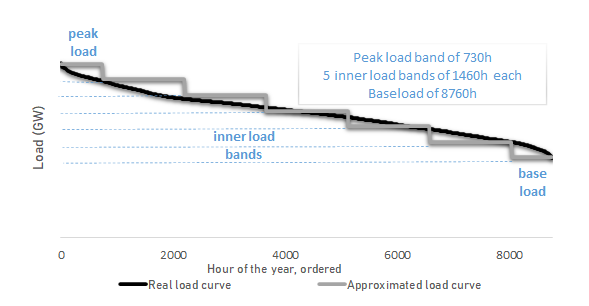
\includegraphics{figures&tables/LDC.png}
    \caption{Load duration curve approximation in IMACLIM-R's electricity module}
    \centering
    \label{fig:LDC}
\end{figure}


To calibrate and reconfigure the load duration curve for each time period, we assume that the ratio of peak load to baseload, (written $bp\_ratio_k$) remains constant and equal to a value supplied by the POLES model.\footnote{
    In principle, this ratio could vary in an exogenous or endogenous manner to integrate, for example, its modification under the effect of policies of demand side management. These policies are not implemented in the current version of the model.
}
The load duration curve approximation associated with a quantity $Q\_elec_k$ of electricity produced in the region $k$, is obtained by solving the equation system, formed by the ratio constancy equation and the constraint equation on the quantity of energy produced, as described in equations \ref{eqn:elecBpRatio} and  \ref{eqn:elecQ}
where $base_k$ and $peak_k$ are the loads required during the base or peak periods respectively.

\begin{dmath}
    \frac{base_k(t)}{peak_k(t)} = bp\_ratio_k
    \label{eqn:elecBpRatio}
\end{dmath}

\begin{dmath}
    Q\_elec_k(t) =
    730*peak_k(t) +
    8760 * base_k(t)  + (8030 + 6570 + 5110 + 3650 + 2190)*\frac{peak_k(t) - base_k(t)}{6} 
    \label{eqn:elecQ}
\end{dmath}

The shape of the load duration curve provides information about the optimal amount of electricity generation capacity needed to meet peak demand and when that capacity should be used during the year. To go further, we need to consider the impact of renewables on the load curve. Residual load duration curves (RLDCs) describe the physical and temporal constraints on electricity demand and supply, including the challenges of integrating variable renewables into power systems.

\paragraph{The residual load duration curve and the challenges to VRE integration.}

Variable renewable energy sources (VRE) such as photovoltaics or wind are inherently non-dispatchable. Therefore, their deployment affects the operation of power systems (\cite{Hirth2015}). Renewable generation increases the need for flexibility in the power system, including dispatchable power to meet peak demand. Indeed, the capacity credit of VRE (the ability to contribute to meeting peak demand in a power system) is low and decreases as the share of VRE in the mix increases.

In order for the technologies to compete on an equal footing (dispatchable vs. variable), we must first adjust the LCOE of VRE to account for its low capacity credit, $i.e.$, the contribution of variable renewables to meeting peak demand. In other words, the "hidden costs" associated with VRE generation are not included in VRE's LCOE. Therefore, we add to VRE's LCOE what is called "integration costs" to calculate VRE's system LCOE, which covers the full economic cost of solar and wind generation. Integration costs measure the costs imposed on the power system to maintain the marginal value of renewable electricity. This includes investments in storage facilities, grid costs, backup costs, etc. Typically, integration costs are divided into three categories, each related to the basic characteristics of renewable energy: uncertainty, locational constraints, and variability.
\begin{itemize}
    \item Balancing costs (uncertainty). They gather actions taken to face VRE output unpredictability, for instance, the cost of intraday trading. Balancing costs tend to zero in absence of forecasting errors on VRE output.
    \item Grid-related costs (locational specificity). Grid-related costs measure the reduction in market value due to the specific generation location of power plants.
    \item Profile costs (variability). Profile costs reflect the marginal value of electricity at different moments in time. As the demand varies through time, profile costs measure the cost of matching this demand with VRE storage devices or conventional backup power.
\end{itemize}

However, estimating value ranges for profile costs and other integration costs is not straightforward. With 20\% renewables in the electricity mix, reported values for integration costs range from €0/MWh to €49.2/MWh (\cite{Heptonstall2021}), reflecting a high degree of uncertainty in integration cost estimates. Indeed, the extent of the loss in the market value of renewable electricity depends on the (in)flexibility of the rest of the electricity system. The more flexible the system, the lower the integration costs. Consequently, estimates of integration costs depend on the underlying energy model and its techno-economic assumptions. The alternative to estimating integration costs would have been to rely on a much more detailed, soft-linked energy system optimization model that includes explicit flexibility solutions for VRE deployment. In this way, we would have lost all the benefits of an embedded power module. Therefore, we chose a synthetic way to account for integration costs through an integration cost markup for PV and wind. The PV (or wind) markup, expressed in \$ per MWh of PV (or wind), is linear with respect to the fraction of wind and PV gross generation and sums to the PV (or wind) electricity generation cost. The parameters $\alpha$, $\beta$, $\gamma$, and $\delta$ are calibrated to reflect typical values of integration costs (in \$ per MWh of VRE generation).

\begin{dmath}
    Markup^{pv}_k(t) = \alpha * Gross\_pv\_share_{k}(t) + \beta * Gross\_wind\_share_{k}(t)
\end{dmath}
\begin{dmath}
    Markup^{wind}_k(t) = \gamma * Gross\_pv_share_{k}(t) + \delta * Gross\_wind\_share_{k}(t)
\end{dmath}
\begin{dmath}
    Integration\_costs_k(t) = Markup^{pv}_k(t) *
    \frac{Gross\_pv\_share_{k}(t)}{Gross\_pv\_share_{k}(t) + Gross\_wind\_share_{k}(t)} +
    Markup^{wind}_k(t) * \frac{Gross\_wind\_share_{k}(t)}{Gross\_pv\_share_{k}(t) + Gross\_wind\_share_{k}(t)}
\end{dmath}


% what to do with the sensitibility analysis?
We still lack robust data to calibrate the integration cost markup parameter and rely on the few existing studies. These parameters will be updated as comprehensive, peer-reviewed studies on integration costs are published. The sensitivity analysis in the figure [forthcoming: sensibility analysis on the markup parameters] shows that the integration cost markup parameter is of great importance for VRE deployment.

The VRE markup is the counterpart of the cost of variable renewables in the rest of the power system. This is captured by a distortion of the residual load duration curve as the share of renewables in the mix increases: the higher the share of renewables, the steeper the residual load duration curve \cite{Ueckerdt2015}. Thus, following the ADVANCE "Variable Renewable Energy integration module project \cite{Ueckerdt2017}, the residual peak load becomes a function of VRE gross generation:

\begin{dmath}
    {peak\_res_{k}}(t) = f(Gross\_wind\_share_{k}(t),Gross\_pv\_share_{k}(t))
    \label{eqn:peakres}
\end{dmath}
with the $f$ a third-order polynom (see Annex for the polynomial coefficients).


This way, $base\_res$ and $peak\_res$ are now determined by Equations \ref{eqn:peakres} and \ref{eqn:elecQres}: Equation \ref{eqn:elecBpRatio} no longer holds. However, Equations \ref{eqn:peakres} and \ref{eqn:elecQres} do not prevent negative residual baseload. Thus, Equation \ref{eqn:elecQres} includes the possibility to adapt if solving the system of equations \ref{eqn:peakres} and \ref{eqn:elecQres} yields negative residual baseload. If for  $nb\_steps$ = 6 (starting case), the residual baseload is negative, the 8760h load band is removed, and the system of equations \ref{eqn:peakres} and \ref{eqn:elecQres} is solved again with one less load band, as shown on Figure \ref{fig:RLDCapprox}. It implies that the conventionnal capacity does not provide a minimum power throughout the year. This way, the residual load curve is always positive and conserves its properties. A version of the residual load duration curve design with a miminum load band (\cite{Ueckerdt2015}) (continuous supply from dispatchable plants throughout the year) is currently under developement.

% adapted from doi: 10.1016/j.renene.2014.08.065 

\begin{dmath}
    Q\_elec\_res_k(t) =
    {peak\_res_k}(t) * 730 +
    {base\_res_k}(t) * {lower\_load\_bands_k} +
    \frac{peak\_res_k(t) - base\_res_k(t)}{nb\_steps_k} * ( \sum inner\_load\_bands_k)
    \label{eqn:elecQres}
\end{dmath}


The residual peak load and the net share (without curtailment) of non-VRE generation in total demand depend on the gross VRE generation. Additionally, the ADVANCE project module was also used to calibrate 1) VRE curtailment and storage losses 2) storage capacity and output as a function of the share of solar PV and wind energy in the mix, the same way the residual peak load does (see equation \ref{eqn:peakres}).

\begin{dmath}
    {curt_{k}}(t) = g(Gross\_wind\_share_{k}(t),Gross\_pv\_share_{k}(t))
    \label{eqn:curt}
\end{dmath}

\begin{dmath}
    {stor\_cap_{k}}(t) = h(Gross\_wind\_share_{k}(t),Gross\_pv\_share_{k}(t))
    \label{eqn:stor_cap}
\end{dmath}

\begin{dmath}
    {stor\_output_{k}}(t) = m(Gross\_wind\_share_{k}(t),Gross\_pv\_share_{k}(t))
    \label{eqn:stor_out}
\end{dmath}




%cite Ueckerdt, Pietzcker et al. from https://fp7-advance.eu/?q=content/variable-renewable-energy-integration-module
\begin{figure}[H]
    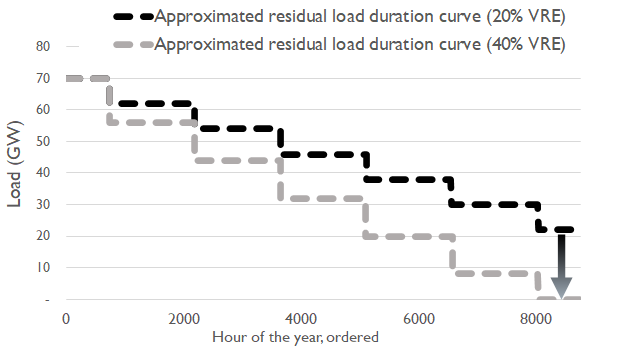
\includegraphics[scale=0.8]{figures&tables/LDC&RLDC.png}
    \centering
    \caption{Illustrative RLDC approximation for 20\% and 40\% net VRE share}
    \label{fig:RLDCapprox}
\end{figure}

In the end, this residual load duration curve design allows representing VRE integration challenges in a compact electricity module such as IMACLIM-R's by relying on the highly resolved Dispatch and Investment Model for Electricity Storage (DIMES)  outputs. Basically, it allows the electricity sector of IMACLIM-R to include the impact of variable renewable energy on the electricity system in a simple, yet robust manner. It captures key mechanisms behind the variable renewable energy penetration challenge and yields consistent projections (see section 7).

\paragraph*{Storage.}
For now, only short-term storage is represented in the electricity nexus: storage capacity, outputs and losses are extracted from the DIMES output (see equation \ref{eqn:stor_cap} and \ref{eqn:stor_out}) and DIMES only optimizes short-term storage. Thus, seasonal (long-term) storage is not included yet in the electricity nexus. An explicit representation of storage capacity needs and ouputs is currently under developement.

\paragraph*{Grid and Transmissions and Distribution Losses.}

Investments in grid infrastructures are not modeled in the electricity module of IMACLIM-R. The extra needs related to VRE deployment are included in the VRE markup. Transmissions and Distribution (T\&D) losses are included in the form of an intra electricity sector input-output coefficient, expressing T\&D losses as a share of total electricity output.
\part*{Modeling investment and dispatch decisions}

\section{Optimal planning of investments under imperfect foresight}

With the compact representation of power generation technologies and the (residual) load duration curve presented above, we have the necessary technical details to model investment decisions in the power sector on an annual basis.
The optimal capacity to meet expected demand over an intermediate time horizon (t+10 by default) is then compared to existing capacity to derive the annual investment plan.
The final investment decision is decomposed into five sequential steps:
\begin{enumerate}
    \item Formulating expectations about future demand and future fuel prices;
    \item Choosing  wind turbine and solar PV  electricity production capacity;
    \item Choosing hydroelectric production capacity;
    \item Projecting the optimal conventional (non-renewable) production capacity to meet domestic demand;
    \item Deciding on the annual investment necessary to move the existing production capacity towards the optimal capacity that has just been calculated
\end{enumerate}

The optimal planning procedure relies on a modified multinonial logit structure (\cite{Clarke1993}), which is an alternative to forward-looking cost optimization in simulation and recursive dynamic Integrated Assessment Models (\cite{GCAM}). The modified multinomial logit structure acknowledges for the fact that determining factors in the investment decision are not modeled, such as individual preferences ($e.g$ for nuclear power) and local variations in electricity generation conditions.
The separate treatment of VRE and hydropower is justified by the special characteristics of these energy sources. A more detailed explanation of these peculiarities is provided below.

\paragraph{Projected demand, fuel prices and carbon tax.}

The optimal installed capacity and level of annual investments are determined using backward-looking expectations of electricity demand growth and  future fossil fuels prices over the coming ten years.

The projected electricity demand for the period $t+10$ in region $k$, written $Q\_elec_k^{anticip}$(t) (in $MWh$), is computed assuming an arithmetic growth of future demand, with $Q\_elec_k$  the final electricity demand of period $t-1$ : 

\begin{dmath}
    Q\_elec_k^{anticip}(t) = Q\_elec_k(t) + (Q\_elec_k(t) - Q\_elec_k(t-1))*10
    \label{eqn:elecQAnticip}
\end{dmath}

Expected electricity demand addressed to conventional (non-renewable) power plants is associated with an anticipated residual load duration curve which is determined using the results from the resolution of the equation system \ref{eqn:peakres}-\ref{eqn:elecQres}.

Current fossil fuel prices are taken as anticipated future prices. Thus, we assume that, given the uncertainty of short-term fluctuations in fossil fuel prices, electricity producers consider current prices to be the best available information 
Regarding the carbon tax on fossil fuels, the IMACLIM-R rationale allows for different beliefs regarding climate policies. By default, the trajectory of the carbon tax is not known. The current carbon tax is projected over the lifetime of the power generation project to calculate its LCOE. Therefore, the current carbon tax is the main climate policy tool. However, it is possible to allow for :
\begin{itemize}
    \item alternative regimes of expectations, $e.g.$ perfect foresight on the carbon tax trajectory
    \item divergent beliefs among actors about the future carbon tax, depending on the level of confidence in climate policy. These divergent beliefs could even be endogenized in future model developments
\end{itemize} 

\paragraph{Determining investments in non-hydroelectric renewable production capacity.}

The investment decision in IMACLIM-R for both renewable and non-renewable technologies is based on a modified multinomial logit (or modified logit). It also accounts for the fact that the cheapest option does not displace more expensive technologies in the electricity market when there is uncertainty, incomplete information, energy security concerns, etc.
The modified multinomial logit choice function takes as input a vector of LCOE (referred to as the choice indicator in the logit framework) and returns a vector of market shares for the corresponding alternatives. The random term is assumed to follow a Weibull distribution such that the market share $S_{k, i}$ for technology $i$ in region $k$ is given by equation \ref{eqn:MMLFVRE}:
With $\gamma$ the logit exponent, $LCOE_{i}$ the LCOE, $\alpha_{k,i}$ the share weight of technology i, and $N$ the number of technological options.
We also assume that the central planner in the electricity market selects the market share for a medium-term horizon (ten years) based on the current costs of the technologies.


\begin{dmath}
    S_{k,i}(t) = \frac{\alpha_{k,}*LCOE_{k,i}^{\gamma}(t)}{\sum_{j=1}^{N} \alpha_{k,j}*LCOE_{k,j}^{\gamma}(t)}
    \label{eqn:MMLFVRE}
\end{dmath}

In the electricity sector of IMACLIM-R, a first logit nest determines the share of variable renewables (wind and solar PV) and the aggregate share of non-variable renewables in total electricity generation. The market share for each non-variable renewable energy is determined by a second logit nest.
The choice indicator for the aggregated dispatchable plants’ share is the lowest LCOE on baseload\footnote{Technologies with limited potential due to resource endowment constraints (hydro, CSP) or social acceptance (nuclear) were excluded from the non-variable renewables choice indicator.}. The weight shares $\alpha_{k,i}$ are calibrated to reproduce 2018 observed market shares for the four VRE technologies (wind onshore, wind offshore, central PV and rooftop PV) and progress thereafter towards equal weighting. Thus, we assume that all non-LCOE factors driving VRE deployment (financial support like feed-in tariffs, national preferences etc.) are declining, electricity generation technologies ending by competing solely based on their economic costs.

The sum of the VRE market shares yields the share of net VRE generation in the total expected electricity demand in region k. The remaining ("residual") demand must be met with dispatchable power plants, including hydropower, CSP and conventional thermal power plant.


As shown in Figure \ref{fig:suminv}, the first logit nest determines the global share of variable renewables from which the residual electricity demand for dispatchable capacity is derived. Once the residual load duration curve is approximated, dispatchable technologies compete for each load band in the second logit nest.

\begin{figure}[H]
    \centerline{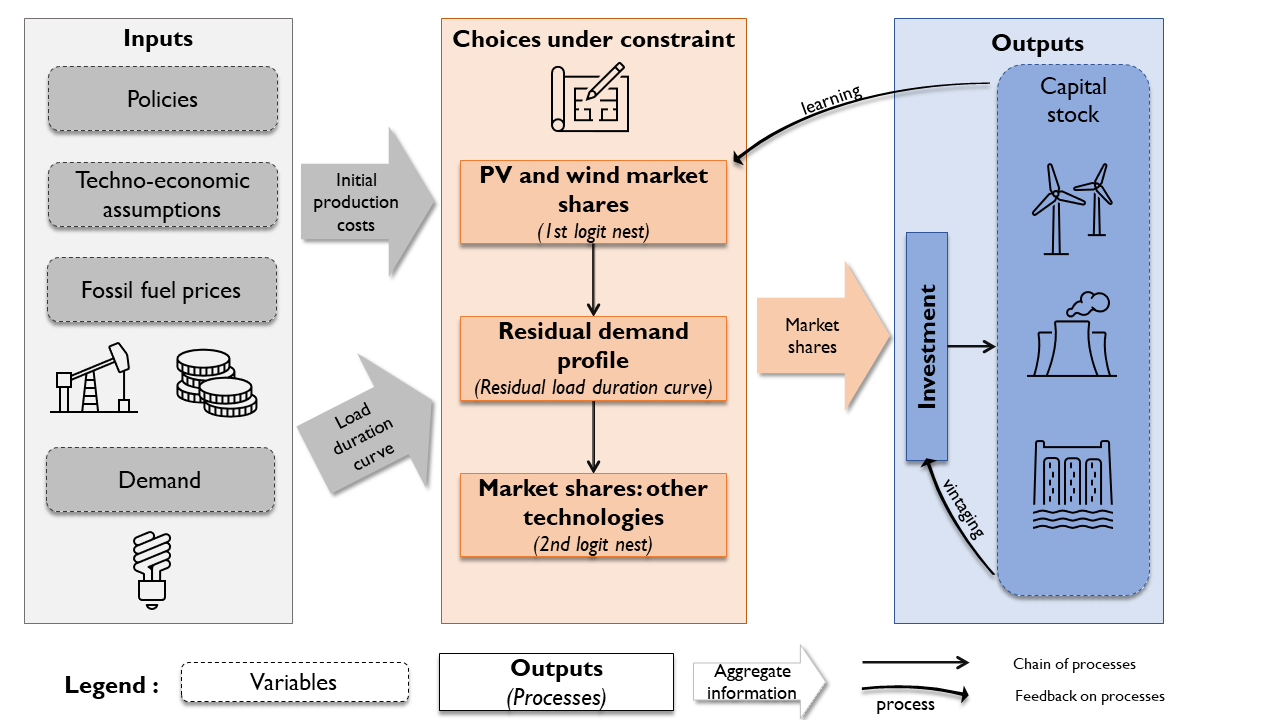
\includegraphics[scale=0.45]{figures&tables/Summary_nexus.png}} %not bad for centering!!
    \caption{Summary of the investment procedure in the electricity sector}
    \label{fig:suminv}
\end{figure}


\paragraph{Investment in hydroelectricity}

Hydropower is treated in a special way because investment in this technology is contrained by the regional physical potential.
In this module, we make no distinction between run-of-river and conventional (dammed) hydropower plants. Therefore, investments in hydropower plants in this module are exogenous and comes from the POLES model (\cite{Keramidas2018}).


\paragraph{Conventional installed production capacity}

Once the optimal share of VRE generation is know, the residual load duration curve is derived following the procedure described in the "Residual load duration curve" section.



Planning the conventional installed production capacity at minimal cost for the period t+10 means determining, for each discrete segment of annual utilization, the cheapest production mix.
Assessing the competitiveness of a technology to satisfy a fixed annual utilization period is done by calculating the discounted total production cost of a
$kW$ over this utilization period.
The corresponding variable, written $LCOE_{H}$, is computed for each load band of width $H$. In other words, the module computes for each conventional technology the levelized cost of producing 1 kW of power for $H$ hours over the plant's lifetime, $H$ corresponding to one of the seven load bands width. When $H$ equals full load hour (8760h), then this metric corresponds to the standard LCOE.

$LCOE_{H}$ includes:

\begin{itemize}
    \item the (annualized) capital cost or construction cost
    \item the fixed total discounted operation and maintenance costs per kWh installed
    \item the variable total discounted operation and maintenance costs per kWh produced
    \item the total discounted fuel costs, calculated using the final price scenarios of the anticipated fossil energies.
    \item  the availability factor, which incorporates planned outages and maintenance
    \item the cost of capital which serves as a proxy for the discount factor
\end{itemize}



Thus, the market share for each load band is derived by a second modified multinomial logit nest where only dispatchable power plants compete. Hydropower generation is removed from the lower bands of the residual load curve because hydropower investments are autonomous and hydropower is dispatched first ($i.e$ in the lower load bands) due to its very low variable cost. The module can determine the required installed capacity of conventional power technologies available for investment to meet the expected electricity demand of t+10 by summing the desired capacity for each load band.

%\paragraph{Capacity markets}

%To account for capacity markets, a reserve margin of 20\% is added to the residual peak load. This strengthen the reliability of the power system in case of unexpected events (e.g. unplanned outages). The reserve margin applies to the residual peak load, which means that the small capacity credit of renewable energy sources is already taken into account. Thus, the reserve margin only increases the demand for dispatchable power plants.

\paragraph{Final investment: minimizing the distance between the optimal production capacity and the installed capacity}

The procedure described in the previous subsection allows us to define at each period $t$  the optimal anticipated production capacity for the period $t+10$. Between t and $t+10$ an investment plan determines the yearly capacity additions needed to reach the optimal $t+10$ capacity.

In the present version of the model, it is not possible to either remove certain production capacity before the end of their lifetime or modify the technologies embodied in the installed plants, $i.e.$ there is no early decommissioning or retrofitting. We thus treat the inertia of the equipment and technologies as if they are utilized for their full lifetime.

Moreover, investments in the electricity sector are constrained by the availability of capital, like any other sector of IMACLIM-R. The composition of the actual investment made is obtained by solving the program that minimizes the distance between optimal investment and available capital. Renewable investment needs are prioritized over conventionnal capacity additions if the available capital cannot satisfy both.
To avoid oversizing capacity, an additional constraint is added to the investment decision in the form of maximum residual peak load coverage. The residual peak load coverage serves as a measure of the grid reliability.

If the existing dispatchable capacity covers the residual peak load beyond a coverage target, the final investment is reduced with regard to the investment determined by matching the residual load duration curve with the optimal market shares from the modified multinomial logit nest. This prevents the electricity module from overinvesting in conventional capacity even if the current capacity is sufficient to meet the residual demand. Such a situation would occur in the case of a sudden fuel switch, for example when coal-fired generation temporarily becomes cheaper than gas-fired generation, resulting in investment in both coal and gas capacity to meet baseload. Note that the final investment is always a non-negative fraction of the optimal investment, $i.e$ $y_{min} > 0$. Variable renewables and CCS are excluded from the investment constraint.

\begin{figure}[H]
    \centerline{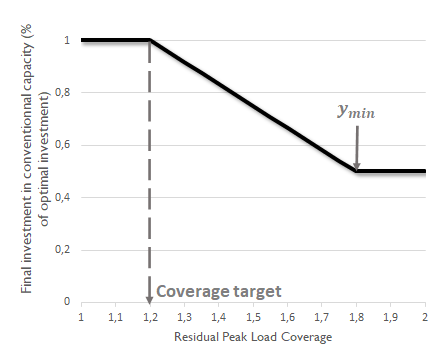
\includegraphics[scale=1]{figures&tables/peak_load_cov.png}} %not bad for centering!!
    \caption{Constraint on investment - residual peak load coverage}
    \label{fig:peakcov}
\end{figure}

These investments create a new generation of capital that marginally changes the composition of installed power capacity for the next static equilibrium. The figure \ref{fig:suminv} summarizes the investment process of the power sector of IMACLIM-R, from the ideal power mix at time $t+10$ to the annual capacity additions.
Based on this newly installed generation capacity and the depreciated capital, the current electricity demand can be met.




\section{Dispatch decision in a compact electricity module}

%Remark: honnestly do we care about this? for non-expert reader the static/dynamic difference is messing up
%"According to IMACLIM-R's architecture, the match between electricity demand and current installed capacity at period t would occur in the static equilibrium. Indeed, the power dispatch is a matter of short term decisions constrained by the existing capital in the electricity sector. However, the integration of the power dispatch into the static equilibrium was considered too complex, and was left in the dynamic module.

%In every region of the model, at the period t the power sector's central planner formulates myopic expectations about electricity demand and fossil fuel prices at t+1. The current VRE installed capacity gives the VRE share for t+1, from which the residual load curve is derived."


%Next, the central planner tries to minimize the variable production cost  to match the residual load. The dispatch occurs according to the merit order of dispatchable technologies.
Once the characteristics of the installed operating capacity for the current period of the model are known, the equilibrium between electricity demand and supply can be found.
Since the model solves the equilibrium in the electricity market annually, the dispatch decision also relies on (residual) load duration curves. Renewable electricity generation at time $t$ is subtracted from total demand because it is not dispatchable.
The use of non-renewable power generation capacity to meet residual demand is done according to the merit order of technologies.
In practice, this means that for each load band (starting with the lower band), the technology with the lowest variable production cost is used until:

%be clearer here? does not seem to be cristal clear, maybe some equations could do the job to represent the availability factor

\begin{itemize}
    \item the power called for exceeds the available production capacity for this technology and the next cheapest installed production capacity is exploited to obtain the additional power or,
    \item the available production capacity of this technology exceed the power demanded for this load duration and the remaining available production capacity will be used to answer demand associated with the load duration that is immediately inferior.
\end{itemize}

\begin{figure}[H]
    \centerline{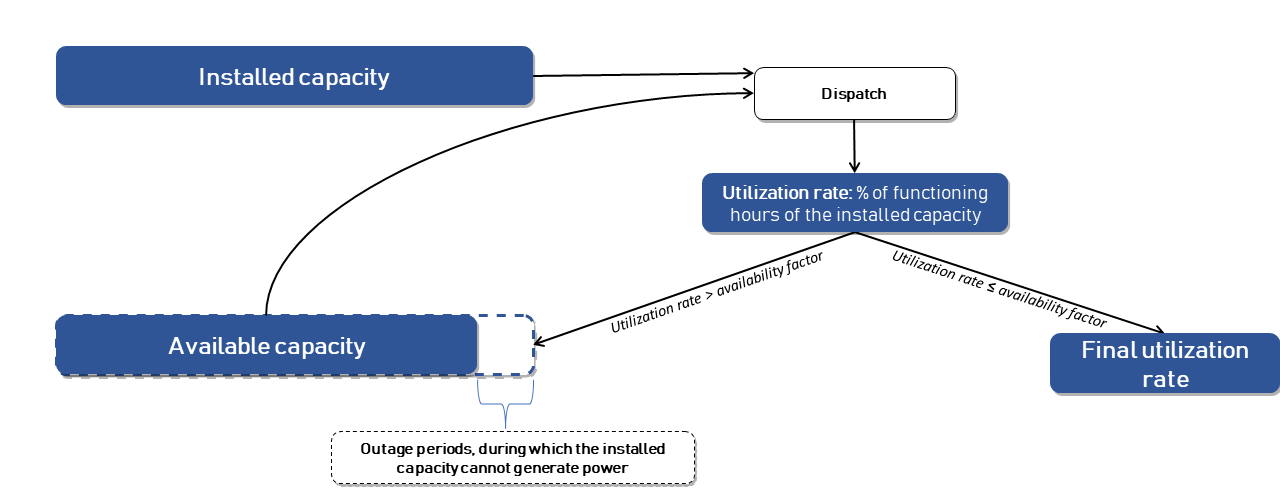
\includegraphics[scale=0.6]{figures&tables/availb.png}}
    \caption{Installed and available capacity during dispatch}
    \label{fig:avail}
\end{figure}


This production cost minimization program allows associating an average annual utilization period (in hours) in each region $k$ and for each technology. For conventional technologies, the utilization rate (the average functioning time of the installed capacity over the 8760 hours of the year) cannot exceed the availability factor. When this occurs for some technologies (e.g. coal units would operate 100\% of the time according to the dispatch procedure, while their availability factor is 85\%), we introduce an available capacity variable to account for outages and maintenance, and perform the dispatch again as shown on Figure \ref{fig:avail}.

\part*{Understanding the role of the electricity sector in a hybrid integrated assessment model: macroeconomic linkage and long term projections}

\section{Linkage between the electricity sector and the macroeconomic core of IMACLIM-R}

The link between the electricity module and the macroeconomic core of IMACLIM-R runs mainly through electricity demand, electricity prices, and fossil fuel prices. Electricity demand and fossil fuel prices are inputs to the electricity nexus: this was discussed in Section 4. The price of electricity is the most important output of the electricity nexus, as it is determined both by the share of fossil fuels in electricity generation (via the input-output coefficients $IC$), by the investment required to provide electricity and the available power generation capacity.
%talk about investment here?
The bottom-up information from the nexus (input-output coefficients, installed capacity per technology) are the building blocks for the electricity sector supply curve in the IMACLIM-R macroeconomic equilibrium. The input-output coefficients $IC$ encapsulate the merit order and dispatch decision from the dynamic module as described above. The final supply curve is used only in the static equilibrium.
The shape of the supply curve determines the market clearing conditions and hence the final electricity price. The electricity sector supply curve (more precisely, the inverse supply curve) can be interpreted as the sum of marginal production costs ($Cm$) plus a sector-specific profit markup ($\pi$), like any sector of IMACLIM-R 
Unless otherwise stated, the electricity sector is assumed to be perfectly competitive. Thus, the markup covers only the costs of investment and capital depreciation. The markup is set prior to market clearing. It is calibrated so that, at current intermediary and final prices, the sum of average electricity generation costs (including investment costs) and the profit markup equals the regional market price of electricity.
Thus, the marginal cost of electricity generation in region $k$ is given by:

\begin{dmath}
    Cm_{k} = \sum_{j}{}pIC_{j,k}*IC_{j,k} + (\Omega_{k}*w_{k})*l_{k}*(1+tax_{k}^{w})
    \label{eqn:Cm}
\end{dmath}
and the electricity price is given by : 

\begin{dmath}
    p_{k} = \sum_{j}{}pIC_{j,k}*IC_{j,k} + (\Omega_{k}*w_{k})*l_{k}*(1+tax_{k}^{w}) + \pi_{k} * p_{k}
    \label{eqn:p}
\end{dmath}
\begin{itemize}
    \item The technical unitary coefficients of production which characterize the electricity sector (quantities of different fuels required to produce a unit of electricity) are determined for coal, gas and liquid fuels ($tech = [coal,gas,et]$) by equation \ref{eqn:IC}.
\end{itemize}


\begin{dmath}
    IC_{tech,elec,k} = \frac{\frac{prod\_elec\_techno_{tech,k}}{rho\_elec_{tech,k}}}{Q\_elec}
    \label{eqn:IC}
\end{dmath}

\begin{itemize}
    \item The marginal cost is increasing with the level of electricity generation through the utilization rate $\Omega_{k} = \frac{Q_{k}}{Cap_{k}}$. Static decreasing returns are assumed in every sector of IMACLIM-R and are associated with lower labor productivity. The electricity sector can not provide more than its annual maximum potential production $Cap_{k}$.
% Note here: in the current version, we should account for the change of global load factor (VRE deployment => lower mean load factor). We could change the 80% target to do so instead of computing with the good Cap (for accounting reasons, the Cap value matters).
% but this wont change much, as the electricity sector is structurally able to produce more electricity
$Cap_{k}$ evolves with electrical power capacity additions.
\end{itemize}

The marginal cost of electricity generation is the aggregate supply curve of the electricity sector used in static equilibrium to balance supply and demand. It incorporates information from investment and dispatch decisions through three elements: the profit markup to cover investment costs, input-output coefficients that reflect dispatch decisions, and potential output as a function of available capacity.

Figure \ref{fig:sumacro} summarises the link between macroeconomic, static equilibriums and the two electricity submodules, investment and dispatch.

\begin{figure}[H]
    \centerline{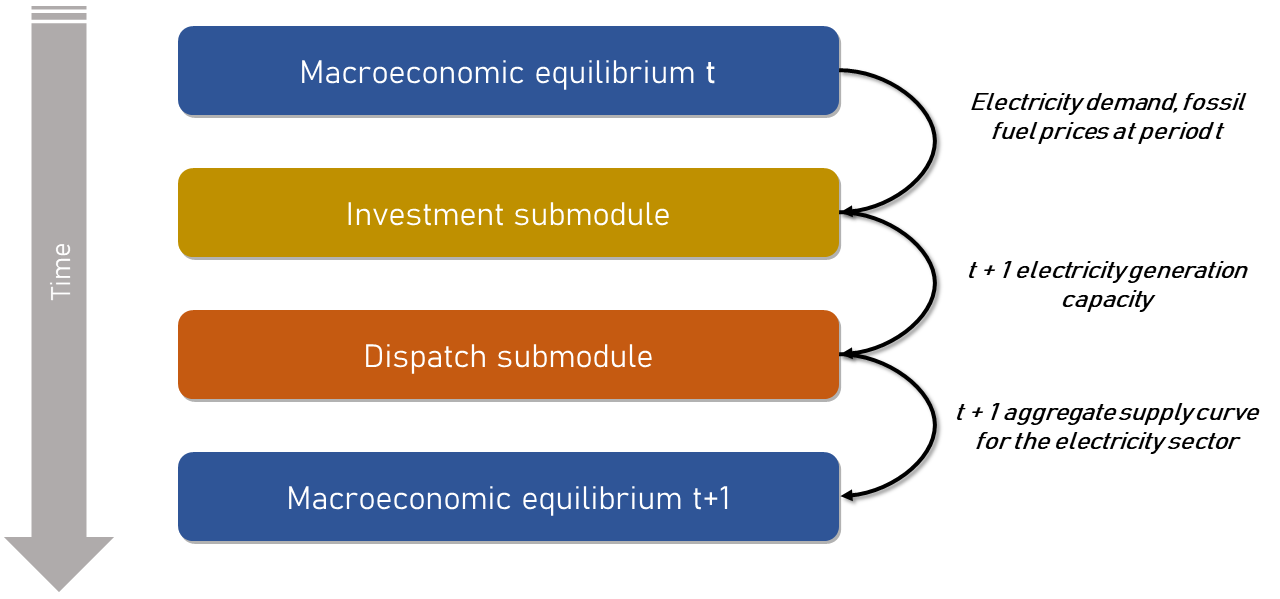
\includegraphics[scale=0.5]{figures&tables/summacro.png}}
    \caption{Summary of the link between macroeconomic static equilibrium and the dynamic submodules of the electricity nexus}
    \label{fig:sumacro}
\end{figure}


\section{Long-term projections for regional power systems}
In this section, we present the main electricity nexus outputs from 2015 to 2100 in two scenarios : a Nationally Determined Contribution scenario, following COMMIT project results (\cite{VanSoest2021}) and a 2°C scenario (1000 GT CO2 budget, 2020-2100). To limit global warming at +2°C by the end of the century, a carbon tax is implemented, starting at 50\$ per ton of CO2 emission in 2020 and reaching 1500\$ per ton in 2100.

\begin{figure}[H]
    \centerline{\includegraphics[scale=0.5]{figures&tables/Prod_doc.png}}
    \caption{World electricity generation by source, NDC (left) and 2°C (right) scenarios}
    \label{fig:Prod}
\end{figure}

\begin{figure}[H]
    \centerline{\includegraphics[scale=0.5]{figures&tables/Msh_doc.png}}
    \caption{World electricity market share by source, NDC (left) and 2°C (right) scenarios}
    \label{fig:Msh}
\end{figure}

\begin{figure}[H]
\centerline{\includegraphics[scale=0.5]{figures&tables/Cap_doc.png}}
    \caption{World installed capacity by source, NDC (left) and 2°C (right) scenarios}
    \label{fig:Cap}
\end{figure}

\begin{figure}[H]
    \centerline{\includegraphics[scale=0.4]{figures&tables/Msh_reg_doc_ndc.png}}
    \caption{World electricity market share by source, NDC scenario}
    \label{fig:Msh_reg_ndc}
\end{figure}

\begin{figure}[H]
    \centerline{\includegraphics[scale=0.4]{figures&tables/Msh_reg_doc_2Deg.png}}
    \caption{World electricity market share by source, 2°C scenario}
    \label{fig:Msh_reg_2deg}
\end{figure}




